\section{Das Fraunhofer ESK}
%------------------------------------------------------------------------

\mode<presentation>{
  \begin{frame}[t] \frametitle{\"Uberblick zum Fraunhofer ESK}
    \begin{itemize}
    \item Fraunhofer ESK steht f\"ur {Fraunhofer-Institut f\"ur \textbf{\usebeamercolor[fg]{structure}E}ingebettete \textbf{\usebeamercolor[fg]{structure}S}ysteme und \textbf{\usebeamercolor[fg]{structure}K}ommunikationstechnik}
    \item kleines Institut: ca. 80 feste Mitarbeiter und etwa 20 Studenten
    \item Standort: M\"unchen
    \item Forschungsschwerpunkt: Verfahren und Methoden der Informations- und Kommunikationstechnik (IKT)
    \item Anwendungen u.a. in:
      \begin{itemize}
      \item Fahrzeugkommunikation und Verkehr
      \item Telekommunikation
      \item Sicherheitstechnik
      \end{itemize}
    \item Gliederung in drei Gesch\"aftsfelder:
      \begin{itemize}
        \item {\usebeamercolor[fg]{structure}Automotive}: Fahrzeugkommunikation
        \item {\usebeamercolor[fg]{structure}Industrial communication}: Automatisierung, Kommunikationssysteme f\"ur Energieversorgung
        \item {\usebeamercolor[fg]{structure}Telecommunication}: \"Ubertragungstechniken, Konnektivit\"at von Kommunikationssystemen
      \end{itemize}
    \end{itemize}
  \end{frame}
}

%------------------------------------------------------------------------
\begin{frame}[t] \frametitle{Gesch\"aftsfeld Automotive}
  \begin{columns}
    \begin{column}{0.55\textwidth}
      \begin{itemize}
      \item Gr\"o\ss tes Gesch\"aftsfeld des ESK (etwa 40 Mitarbeiter)
      \item arbeitet an L\"osungen um die wachsenden Anforderungen an Fahrzeuge (Sicherheit, Flexibilit\"at) zu erf\"ullen:
        \begin{itemize}
          \item bessere Vernetzung von Fahrzeugen
          \item Kommuninkationssysteme f\"ur neuartige Fahrzeugkonzepte (bspw. Elektromobilit\"at)
        \end{itemize}
      \end{itemize}
    \end{column}
    \begin{column}{0.4\textwidth}
      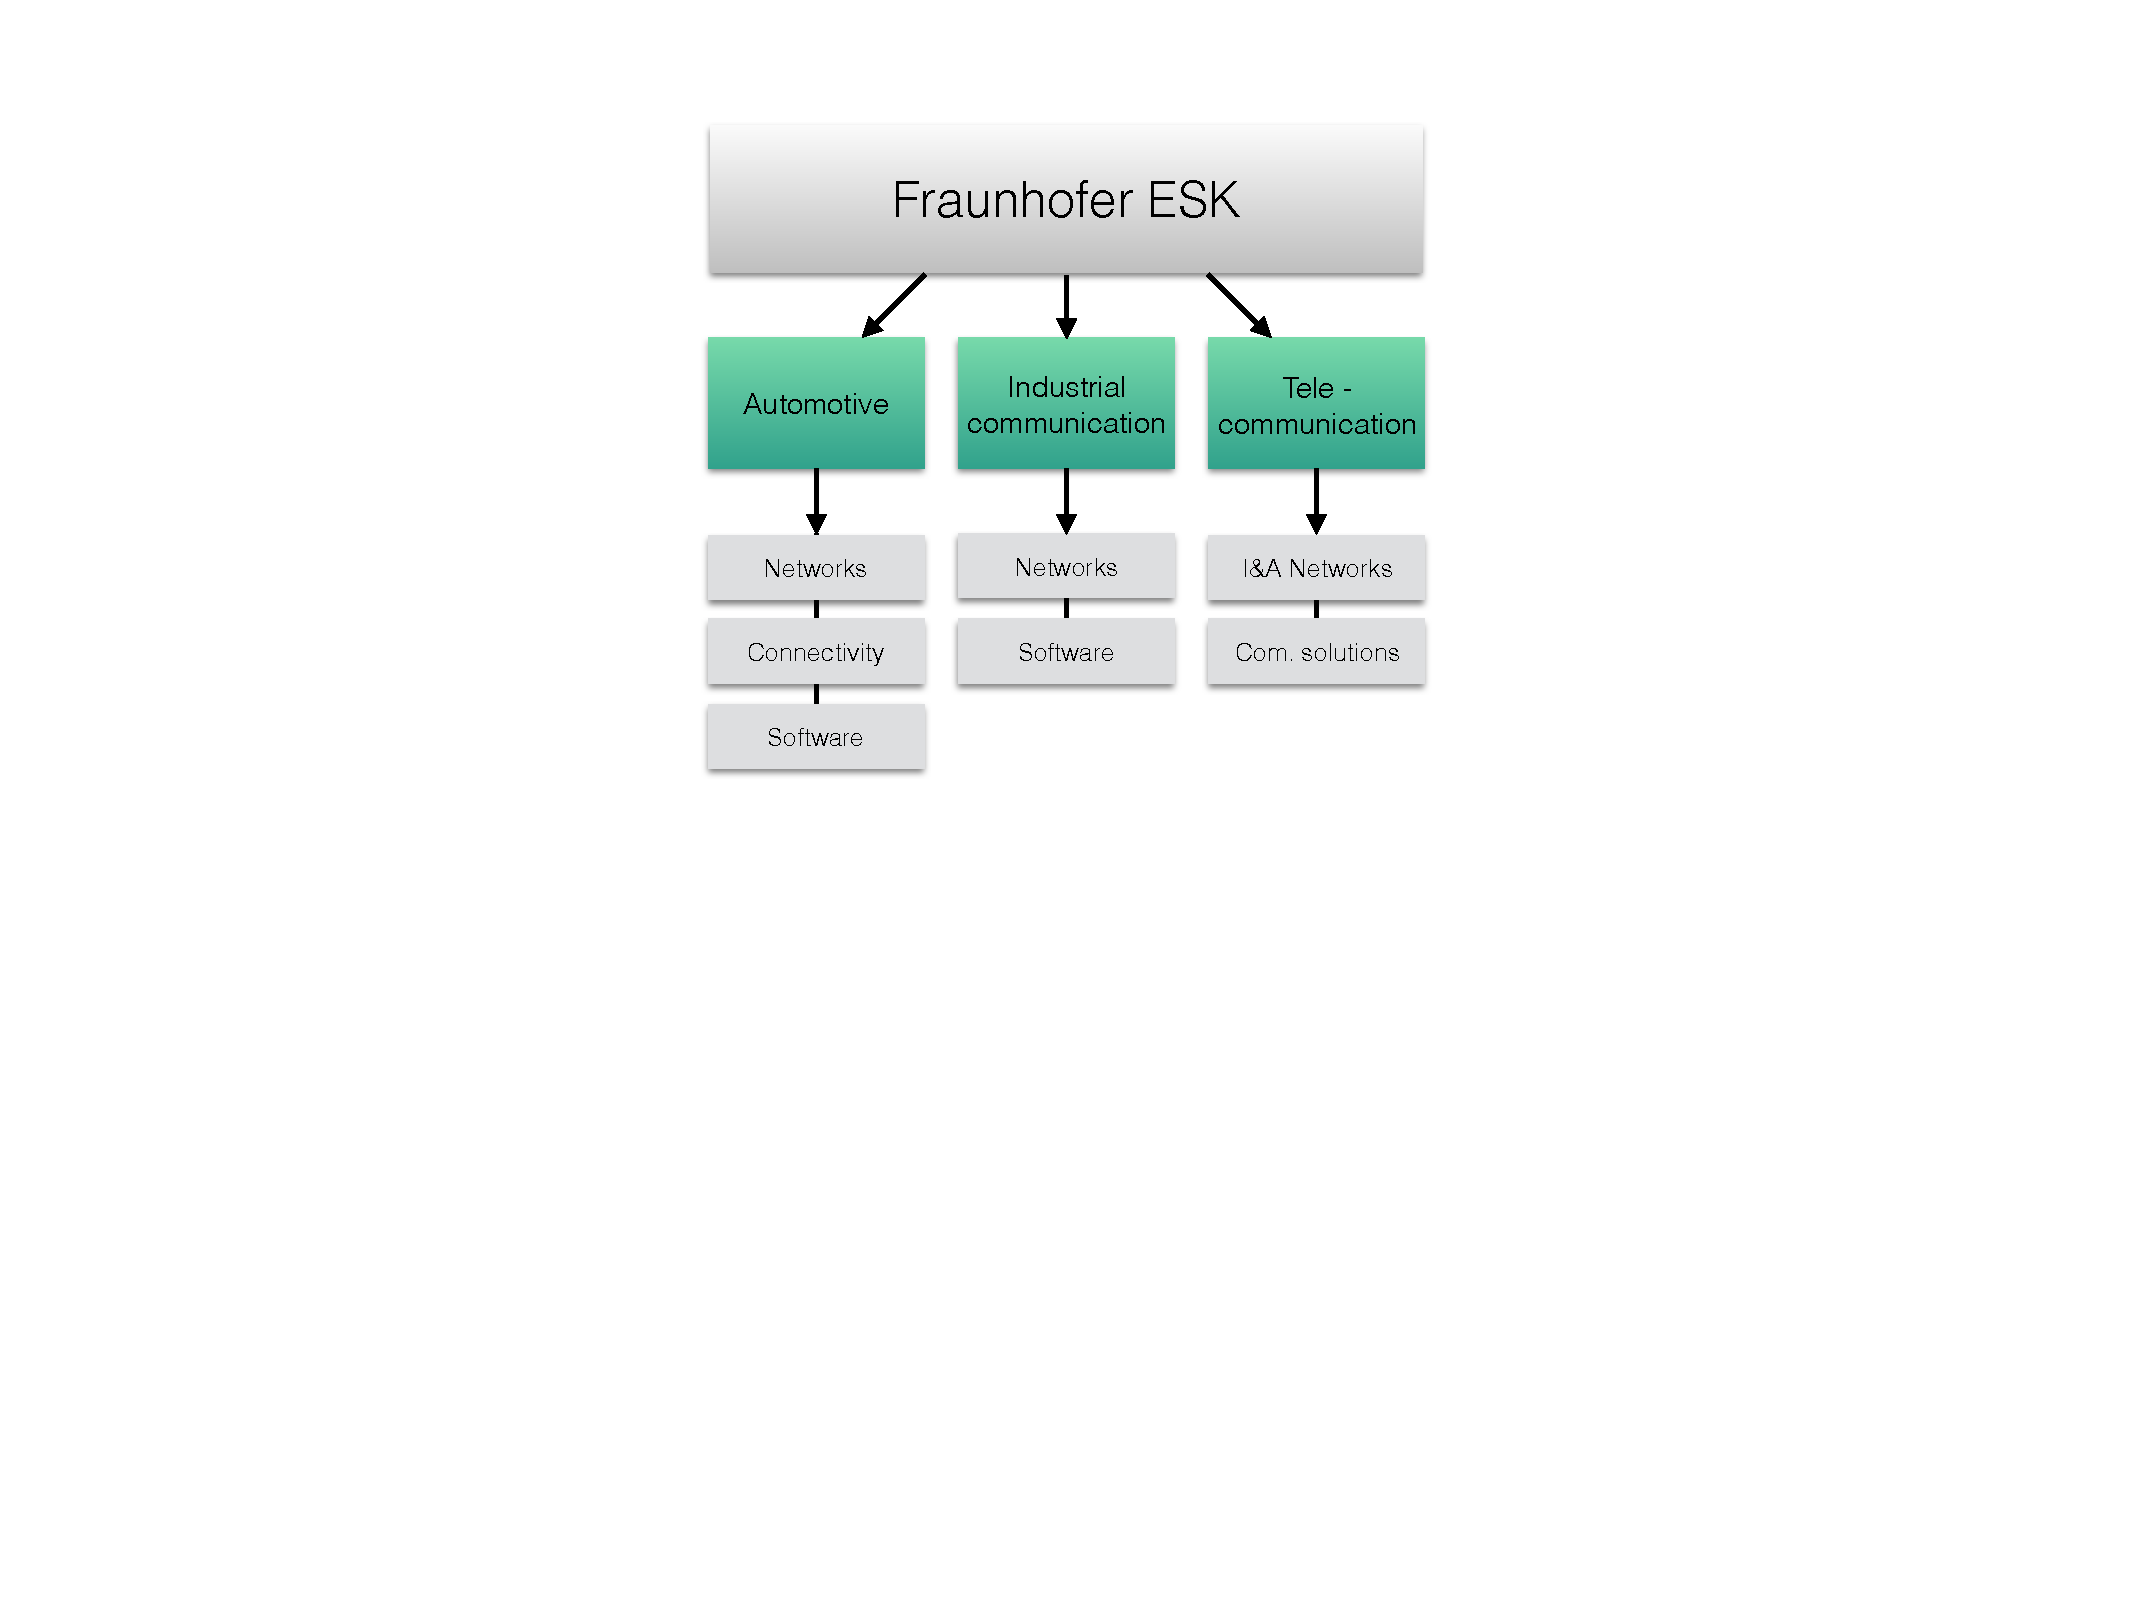
\includegraphics[width=1\textwidth]{pics/chartFraunhofer}
    \end{column}
  \end{columns}
  \begin{itemize}
  \item Automotive Connectivity: Entwicklungen zur Vernetzung von Fahrzeugen untereinander und mit der Umwelt (sog. Car-to-X Kommunikation, kurz C2X) zur Vermeidung von Unf\"allen und Staus
    \begin{itemize}
      \item Datenaggregation und -weiterleitung
      \item Simulationen
      \item Entwicklung von Software-Frameworks
    \end{itemize}
  \end{itemize}
\end{frame}
